\chapter{恒星与夜空}\label{ch:g5:stars-night-sky}

远离城市灯火，在晴朗无月的夜晚，夜空
中密布着成千上万的星光，有的微弱，有的耀眼，有白色的，
也有橙色的。水手依它们辨别方向，农民依它们安排播种，
每门科学都始于对它们的惊叹。它们究竟是什么？为何
在我们入睡时，它们仍然那样有序地在头顶转动？

\section{什么是恒星}

\begin{example}[数不清的太阳]\label{ex:g5:stars-night-sky:suns}
每颗恒星都是一个太阳：一个炽热发光的巨大气团，
自身发出光芒。许多恒星的威力比我们的太阳还要强大。它们
之所以看起来只是渺小的光点，原因只有一个：距离。太阳是我们的近邻恒星；
其余恒星则远得多。即使是光——这位瞬间就能穿过一间屋子的“冠军”，
从最近的一颗恒星来到这里，也要走上\emph{数年}的路程。
夜空就是一群太阳，
因距离而缩小，化作闪烁的光点。
\end{example}

\begin{omfigure}
\begin{tikzpicture}[scale=0.85]
  \fill[omThm] (1.1,1.4) circle (0.4);
  \foreach \a in {0,45,...,315} {
    \draw[omThm] (1.1,1.4) ++(\a:0.55) -- ++(\a:0.22);
  }
  \node[below, font=\small] at (1.1,0.75) {近处的一盏灯};
  \fill[omThm] (8.6,1.4) circle (0.07);
  \node[below, font=\small] at (8.6,0.75)
    {远处道路上的同一盏灯};
  \node[above, font=\small] at (5.3,2.3)
    {距离使任何光都变成光点};
\end{tikzpicture}

{\small 同一盏路灯，近看与远看：亮度随距离减弱，
恒星就是远在一切道路之外的灯。}
\end{omfigure}

\begin{omfigure}
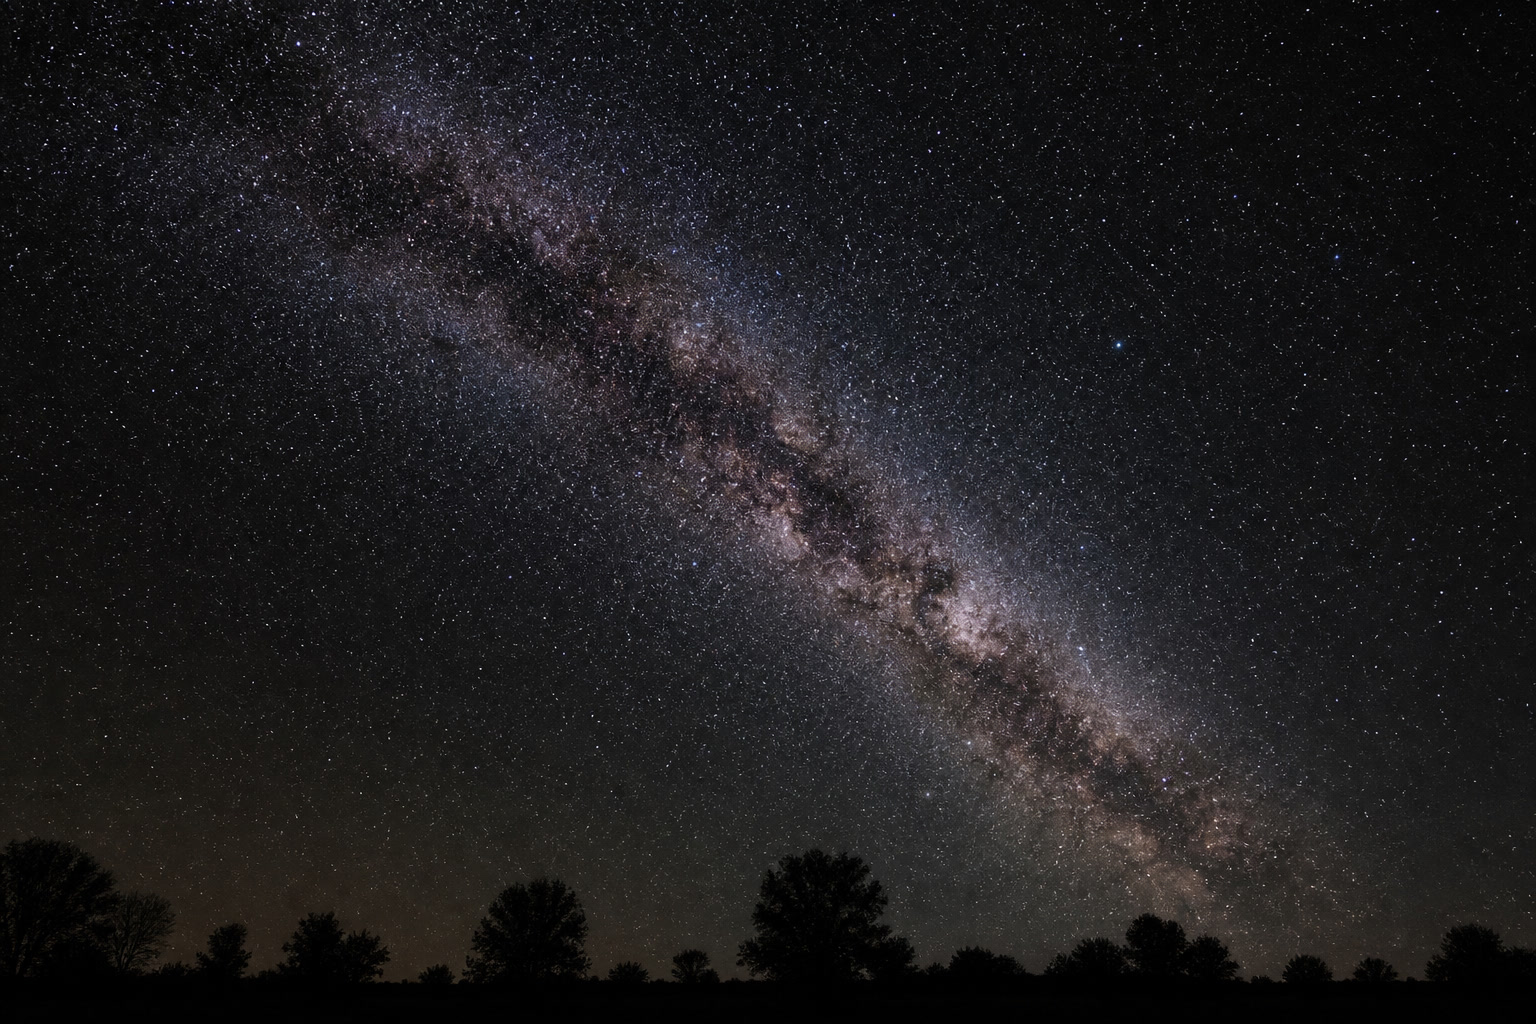
\includegraphics[width=0.58\linewidth]{images/book1/ai/g5-stars-night.jpg}

{\small 远离城镇的漆黑夜空：成千上万颗太阳，以及横贯天空、柔和的银河光带。}
\end{omfigure}

\begin{example}[恒星的颜色]\label{ex:g5:stars-night-sky:colors}
仔细看，这些光点并非都是白色的：有的呈橙红色，
有的像太阳一样呈黄色，有的呈蓝白色。颜色在这里传递的是关于温度的信息，
其规律与水龙头、颜料罐的颜色习惯恰好相反：橙色的恒星是这一家族中\emph{温度最低}的，
而蓝白色的恒星最热，远比太阳还热。
一块发红的炭与一把白热的钢刀，
在地球上讲的也是同一个道理：
温度越高，光越偏白。
\end{example}

\begin{remark}[恒星白天去了哪里]\label{rem:g5:stars-night-sky:daytime}
恒星从未离开。正午时分，它们与午夜一样，依然在你头顶闪耀，
只是白天的天空充满了被空气散射的阳光，
形成一片蓝色的强光，远比任何光点都亮。烛光
在篝火旁是看不见的。太阳落山，强光散去，
夜空中这群常驻的“居民”便又清晰可见了。
\end{remark}

\section{由恒星组成的地图}

\begin{definition}[星座]\label{def:g5:stars-night-sky:constellation}
称由若干颗亮星组成、有名字的图案为\emph{星座}\index{星座}，
例如猎户、天鹅、大熊，是古代观星者为绘图和帮助记忆而创造的。
同一星座中的恒星其实并不相邻，
它们只是从地球上看去才恰好排成一线。
但这些图案十分稳定：你的祖父母所认识的，
正是今天我们看到的同样图形。
\end{definition}

\begin{method}[寻找北极星]\label{met:g5:stars-night-sky:northstar}
夜空提供了一个免费的指南针：
\begin{enumerate}
  \item 找到北斗七星——七颗亮星，形如一把长柄勺，
        全年都很容易找到；
  \item 取勺子前缘的两颗星——即
        \emph{指极星}；
  \item 沿两星的连线向前延长，
        约为两星间距的五倍远；
  \item 落点处那颗不起眼的星，即为
        \emph{北极星}\index{北极星}——从它向下悬挂一根铅垂线，
        垂至地平线，那一方向便是北方。
\end{enumerate}
用指南针核对一下：指针与恒星所指的方向一致。水手们
几个世纪以来，都把性命押在这份一致上。
\end{method}

\begin{omfigure}
\begin{tikzpicture}[scale=0.85]
  % the seven stars of the Dipper: handle, then bowl
  \foreach \x/\y in {0.16/3.59, 1.07/3.03, 1.79/2.53, 2.51/2.02,
      1.82/1.32, 2.60/0.60, 3.40/1.28} {
    \fill[omExo] (\x,\y) circle (0.09);
  }
  \draw[thin, omExo] (0.16,3.59) -- (1.07,3.03) -- (1.79,2.53)
    -- (2.51,2.02) -- (1.82,1.32) -- (2.60,0.60) -- (3.40,1.28)
    -- (2.51,2.02);
  % the pointers' line, five spacings out to the North Star
  \draw[dashed, omThm, -Stealth] (3.40,1.28) -- (6.25,3.71);
  \fill[omThm] (6.60,4.00) circle (0.13);
  \node[right, font=\small, omThm] at (6.85,4.00) {北极星};
  \node[below, font=\small] at (3.1,0.12)
    {北斗七星及两颗指极星};
  \node[right, font=\small] at (5.35,2.15)
    {沿指极星连线的五个间距};
\end{tikzpicture}

{\small 夜空的路标：北斗的两颗指极星
笔直指向北极星。}
\end{omfigure}

\section{转动的天空}

\begin{proposition}[天空绕北极星转动]\label{prop:g5:stars-night-sky:wheel}
整夜里，满天的星星
沿大圆缓缓转过天空——全都绕着一个几乎静止的点，
即北极星。天上并没有什么真的如此规整地运动，
那是我们脚下的地球在自转，正如它带着太阳掠过白天的天空。
北极星几乎不动，是因为它恰好立在
地球自转轴的延长线上——这正是自转唯一
不去搅动的方向。
\end{proposition}

\begin{omfigure}
\begin{tikzpicture}[scale=0.85]
  \fill[omThm] (5.5,3.4) circle (0.11);
  \node[above, font=\small] at (5.5,3.6) {北极星};
  \foreach \r in {0.9, 1.7, 2.5} {
    \draw[omExo, thick] (5.5,3.4) ++(-35:\r) arc (-35:215:\r);
  }
  \foreach \r/\a in {0.9/40, 1.7/130, 2.5/75} {
    \fill[omExo] (5.5,3.4) ++(\a:\r) circle (0.08);
  }
  \draw[thick] (1.5,0.6) -- (9.5,0.6);
  \node[below, font=\small] at (5.5,0.35)
    {地平线 --- 长曝光所绘的夜空};
\end{tikzpicture}

{\small 把相机对准北极星，让它整夜
凝视夜空：每颗星都绕着那个静止的点画出一道弧。
天空的转动就是地球自转，从内部看到的样子。}
\end{omfigure}

\begin{example}[星星之城]\label{ex:g5:stars-night-sky:milkyway}
在最黑的夜晚，一条淡淡的乳白色光带横跨
天空：\emph{银河}\index{银河}。双筒望远镜能把这片乳白
化为真实：无数星星，暗弱而密集，
肉眼难以分辨。这是我们的家乡星城，从内部看去的样子——
一座扁平、旋转的星岛，恒星多过海滩上的沙粒，
而太阳则住在一处安静的郊区。你用肉眼能看到的每一颗星，
都是这座城里的邻居。
\end{example}

\begin{remark}[继续仰望]\label{rem:g5:stars-night-sky:lookup}
天文学是最古老的科学，也是唯一一门实验室
每个晴朗的夜晚都免费开放。一条毯子，一处远离路灯的暗处，
再加上耐心等待眼睛适应黑暗——
这就是全部装备。北斗七星、北极星、一两颗
行星与银河，便是一次很好的初次探索；
星光背后更深的规律，
数年之后，在本课程接近尾声时，将让你做好充分准备。
\end{remark}

\section{练习}

\begin{exercise}[$\star$]\label{exo:g5:stars-night-sky:1}
什么是恒星？许多恒星比太阳还亮，
为什么它们看上去却像一个个小光点？
\end{exercise}

\begin{exercise}[$\star$]\label{exo:g5:stars-night-sky:2}
正午时星星还在天上吗？为什么我们看不见它们？
\end{exercise}

\begin{exercise}[$\star$]\label{exo:g5:stars-night-sky:3}
一颗橙色恒星和一颗蓝白色恒星并排发光，哪一颗更热？
生活中有哪种光也能说明同样的颜色道理？
\end{exercise}

\begin{exercise}[$\star$]\label{exo:g5:stars-night-sky:4}
什么是星座？星座中的星星真的彼此靠得很近吗？
\end{exercise}

\begin{exercise}[$\star$]\label{exo:g5:stars-night-sky:5}
请一步步描述，怎样从
北斗七星找到北极星。
\end{exercise}

\begin{exercise}[$\star$]\label{exo:g5:stars-night-sky:6}
北极星在转动的天空中的位置有何特别之处，
它代替了哪种日常仪器？
\end{exercise}

\begin{exercise}[$\star$]\label{exo:g5:stars-night-sky:7}
星星整夜沿整齐的圆周转动。真正在
转动的是什么？同样的转动还在白天的天空中
呈现出什么？
\end{exercise}

\begin{exercise}[$\star$]\label{exo:g5:stars-night-sky:8}
横跨最暗夜空的乳白色光带，用双筒望远镜看时
原来是什么？它究竟又是什么？
\end{exercise}

\begin{exercise}[$\star\star$]\label{exo:g5:stars-night-sky:9}
整夜无人看管的相机对准北极星，记录下
一圈圈的圆弧；若改对准东方地平线，则记录下升起的
倾斜线条。试用同一个自转的地球解释这两幅照片。
\end{exercise}

\begin{exercise}[$\star\star$]\label{exo:g5:stars-night-sky:10}
一名遇难的水手在晴朗的夜晚，既没有指南针，也没有手机——
也不着急。试解释天空如何为她提供方向，
并且只要耐心等待，还能提供时钟。（本章两个要点，同一片转动的天空。）
\end{exercise}

\begin{exercise}[$\star\star$]\label{exo:g5:stars-night-sky:11}
遥远恒星的光要经过数年才能到达你的眼睛。
今晚你看着那颗星时，看到的是它
\emph{此刻}的样子吗？你实际上看到的是什么——为何这一点
使每台望远镜都成为一种时光机？
\end{exercise}
